% Capitolo 3: Apparato sperimentale

\section{Panoramica del setup}
\label{sec:panoramica-setup}

L'apparato opera in configurazione di trasmissione su rotaia ottica. Lo schema esteso è:
\begin{equation}
\text{Sorgente} \;\longrightarrow\; \text{Campione} \;\longrightarrow\; \left[\,\lambda/4\,\right] \;\longrightarrow\; \text{Analizzatore} \;\longrightarrow\; \text{Sensore}
\label{eq:schema-ottico}
\end{equation}
dove la lamina $\lambda/4$ viene inserita solo per la determinazione di $S_3$. La \cref{fig:setup-foto} mostra due viste dell'apparato assemblato.

\begin{figure}[H]
    \centering
    \subfloat[Vista da sorgente a sensore]{
\includegraphics[width=0.48\textwidth]{Images/setup/vista_NE.png}\label{fig:vista_NE}}
    \hfill
    \subfloat[Vista da sensore a sorgente]{
\includegraphics[width=0.48\textwidth]{Images/setup/vista_NW.png}\label{fig:vista_NW}}
    \caption{Fotografie dell'apparato sperimentale assemblato sulla rotaia ottica Optosci.}
    \label{fig:setup-foto}
\end{figure}


\section{Componenti ottici}
\label{sec:componenti-ottici}

L'apparato è montato su una rotaia ottica Optosci con cavalieri scorrevoli, che garantisce l'allineamento dei componenti lungo un asse ottico comune e la riproducibilità del posizionamento tra sessioni di misura. La sorgente luminosa è il display di un tablet Samsung Galaxy Tab S7 FE, impostato su schermata bianca alla massima luminosità. Il pannello LCD emette luce bianca a banda larga attraverso un polarizzatore integrato: la luce in uscita è già polarizzata linearmente con asse orientato approssimativamente in verticale in configurazione landscape, il che rende il display una sorgente estesa a stato di polarizzazione ben definito. L'analizzatore è un polarizzatore lineare Optosci di forma circolare, montato su supporto rotante calibrato con risoluzione angolare sufficiente per i passi di \SI{10}{\degree} previsti dal protocollo; un rapporto di estinzione elevato garantisce che la modulazione dell'intensità trasmessa segua fedelmente la legge di Malus. Per integrare i dispositivi nella rotaia sono stati realizzati supporti personalizzati mediante stampa 3D in PLA.

\subsection{Lamina \texorpdfstring{$\lambda/4$}{lambda/4} zero-order}
\label{subsec:lamina-qwp}

Per la determinazione del parametro $S_3$ viene utilizzata una lamina quarto d'onda Optosci di tipo \emph{zero-order}, progettata per la lunghezza d'onda di $\SI{633}{\nano\meter}$. Il materiale birifrangente della lamina non è dichiarato dal costruttore e resta ignoto: nelle analisi spettrali che seguono il quarzo cristallino compare unicamente come modello di dispersione di riferimento, ben caratterizzato in letteratura, e non come materiale accertato delle lamine. Rispetto a una lamina multi-ordine, la dipendenza dalla lunghezza d'onda è più debole, proprietà importante dato che il sensore opera simultaneamente sui tre canali colore. Il ritardo effettivo alla lunghezza d'onda $\lambda$ del canale in esame è:
\begin{equation}
\delta(\lambda) = \frac{\pi}{2} \cdot \frac{\SI{633}{\nano\meter}}{\lambda}
\label{eq:qwp-geometrico}
\end{equation}
La correzione per questo effetto cromatico è descritta nel \cref{ch:analisi}.


\section{Sensore e acquisizione RAW}
\label{sec:sensore}

Il rivelatore è la fotocamera principale di uno smartphone Samsung Galaxy S24, con sensore CMOS da circa 10 megapixel effettivi, obiettivo a focale $\SI{7.0}{\milli\meter}$ (equivalente $\SI{69}{\milli\meter}$), apertura $f/2.4$ e profondità di acquisizione fino a 12~bit per canale.

% TODO: check (figura Bayer da Wikimedia Commons inserita da AI 2026-05-21, lic. CC BY-SA 3.0)
Il sensore è ricoperto da una matrice di Bayer con disposizione RGGB (\cref{fig:bayer}). In condizioni normali di utilizzo, il processore di immagini dello smartphone applicherebbe demosaicizzazione, bilanciamento del bianco, correzione della gamma e compressione, elaborazioni che distruggono la linearità del segnale. Per questo motivo, tutte le acquisizioni sono effettuate in formato RAW (DNG, \emph{Digital Negative}), che fornisce il segnale grezzo a 12~bit con risposta proporzionale all'intensità incidente, condizione necessaria per l'applicazione della legge di Malus. La dinamica di $2^{12} = 4096$ livelli per canale garantisce una risoluzione sufficiente per distinguere variazioni sottili nell'intensità polarizzata, e ciascun canale colore (R, G, B) può essere estratto e analizzato indipendentemente, consentendo di fatto un'analisi polarimetrica a tre lunghezze d'onda con un singolo sensore. L'acquisizione viene controllata da remoto via USB tramite il software \texttt{scrcpy}, per evitare vibrazioni indotte dal contatto con il dispositivo.

\begin{figure}[H]
    \centering
    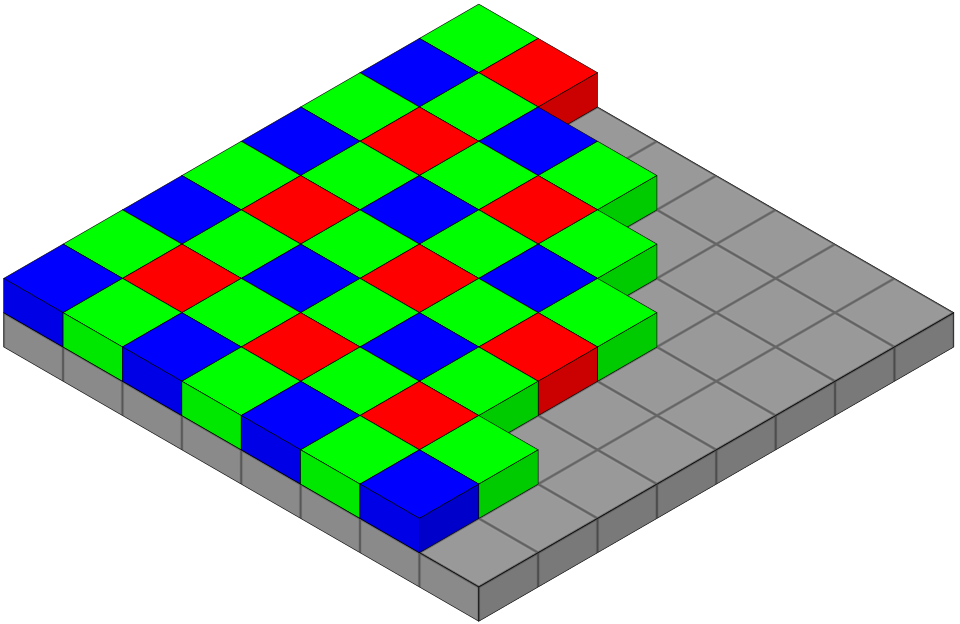
\includegraphics[width=0.45\textwidth]{Images/bayer_pattern.png}
    \caption{Disposizione della matrice di filtri di Bayer in configurazione RGGB: ogni cella di $2\times2$ fotositi comprende un filtro rosso, uno blu e due verdi. Estraendo dal RAW solo i fotositi di un dato colore si ottiene una mappa di intensità per quel canale, alla base dell'analisi polarimetrica a tre lunghezze d'onda. Immagine di Cburnett (Wikimedia Commons), licenza CC BY-SA 3.0.}
    \label{fig:bayer}
\end{figure}


\section{Protocollo di acquisizione}
\label{sec:protocollo}

\subsection{Acquisizione per i parametri di Stokes lineari (\texorpdfstring{$S_0$, $S_1$, $S_2$}{S0, S1, S2})}
\label{subsec:acquisizione-lineari}

La determinazione dei parametri di Stokes lineari $S_0$, $S_1$ e $S_2$ si basa sull'acquisizione di una sequenza di 36 immagini RAW, corrispondenti a 36 posizioni angolari dell'analizzatore distribuite uniformemente tra \SI{0}{\degree} e \SI{350}{\degree} con passo di \SI{10}{\degree}. Con 36 misure per 3 incognite, il sistema è fortemente sovradeterminato: i parametri di Stokes vengono estratti mediante la matrice pseudo-inversa di Moore-Penrose, come descritto nel \cref{ch:analisi}. La sovradeterminazione migliora la robustezza statistica del fit, riducendo l'effetto del rumore del sensore. Gli angoli nominali dell'analizzatore entrano direttamente nella ricostruzione; l'orientazione del sistema di riferimento polarimetrico viene fissata a valle, allineando gli assi alla direzione di polarizzazione del display (\cref{ch:analisi}), mentre la convenzione di elicità è ancorata al segno di $S_3$ (\cref{ch:teoria}).

\subsection{Acquisizione per il parametro di Stokes circolare (\texorpdfstring{$S_3$}{S3})}
\label{subsec:acquisizione-s3}
% TODO: check (cite manuale aggiunta da AI 2026-05-21)
Per la determinazione di $S_3$, secondo il metodo descritto nel manuale di laboratorio del corso di Fisica Sperimentale del Politecnico di Milano~\cite{manuale_polarizzazione}, si acquisiscono due immagini aggiuntive inserendo la lamina $\lambda/4$ nel percorso ottico tra il campione e l'analizzatore: una con l'asse veloce orientato a $+45^\circ$ rispetto all'asse dell'analizzatore, e una a $-45^\circ$. Il parametro $S_3$ viene calcolato dalla differenza delle intensità misurate nelle due configurazioni, con la correzione per la dispersione cromatica della lamina descritta nella \cref{subsec:lamina-qwp}; l'ordine delle due immagini nella differenza fissa il segno di $S_3$ secondo la convenzione di elicità adottata (\cref{sec:determinazione-s3}).

Tutti i parametri di esposizione vengono fissati manualmente e mantenuti costanti per l'intera sessione (\cref{tab:costanti-radiometriche}). Le acquisizioni avvengono in oscurità ambientale, con la sola illuminazione del display del tablet, per eliminare contributi di luce parassita. I parametri di Stokes normalizzati ($s_i = S_i/S_0$) sono per definizione indipendenti dall'intensità assoluta della sorgente, eliminando la necessità di una calibrazione assoluta; la variabilità residua è dominata dal rumore del sensore, ridotto dal downsampling e dalla sovradeterminazione del sistema lineare.

\begin{table}[H]
    \centering
    \caption{Costanti radiometriche impostate durante l'acquisizione.}
    \label{tab:costanti-radiometriche}
    \begin{tabular}{ll}
        \hline
        \textbf{Parametro} & \textbf{Valore} \\
        \hline
        Formato di acquisizione & DNG (Linear RAW, 12~bit/canale) \\
        Lunghezza focale & $\SI{7.0}{\milli\meter}$ ($\SI{69}{\milli\meter}$ eq.\ 35~mm) \\
        Apertura & $f/2.4$ (fissa) \\
        Tempo di esposizione & $1/\SI{90}{\second}$ \\
        Sensibilità ISO & 50 \\
        Bilanciamento del bianco & D65 / Standard Illuminant A \\
        \hline
    \end{tabular}
\end{table}

Il protocollo produce, per ogni sessione di misura, un dataset di 38 immagini RAW: 36 per la ricostruzione dei parametri di Stokes lineari e 2 per il parametro circolare. Il capitolo seguente presenta i campioni selezionati per la validazione dell'apparato, scelti per coprire i tre fenomeni polarimetrici descritti nel \cref{ch:teoria}.
